\subsection{Results and Analysis}

\begin{todolist}
\item describe more in figure \ref{Plot variance default and Local Cost}
\item analysis instead of describing
\item add the figures above (python notebook) for analysis
\item describes how alternating data lead to different result(s).
\end{todolist}

The section \ref{Development Process section} discusses the configurations of the experiment. 
We summarise the experiment results as the table:
\begin{center}
    \begin{tabular}{|| c c c ||}
        \hline
        Ansatz      & Method                                & Variance of gradients \\[0.5ex] 
        \hline \hline
        NLocal      & None                                  & Decay                 \\
        \hline
        TwoLocal    & None                                  & Decay                 \\
        \hline
        NLocal      & Local Cost Function, Shallow circuit  & Sustain               \\
        \hline
        TwoLocal    & Local Cost Function, Shallow circuit  & Sustain               \\
        \hline
    \end{tabular}
\end{center}

\almarginpar{First of all, the table above has no caption or number. Then I do not understand the method "None" clearly this is impossible - you mean global cost and long circuit perhaps? Then, which two ansatze w are talking about first?}
The two ansatzes' gradient variances decay as expected for the default setting.
As the number of qubits scales up, the variance values decay exponentially. 
The figure \ref{Plot ansatzes variance default} shows the results of the two ansatzes in this configuration.
This result indicates that the cost function landscape becomes flatter and flatter. 
Eventually, the gradient would reach a near-zero value across a large plateau, which would be inefficient for any gradient-based optimization algorithm to train the model.
We discussed this phenomenon in Section \ref{Barren Plateaus section}.


\begin{figure}
    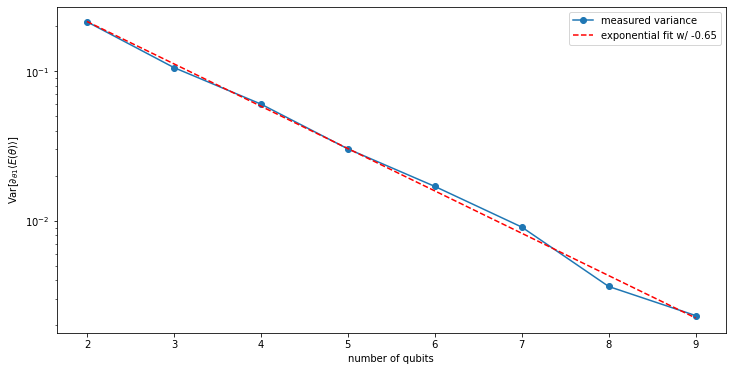
\includegraphics[width=\textwidth]{Artefact/Appendices/NLocalDefault.png}
    \centerline{a) NLocal Ansatz gradient variance values}
    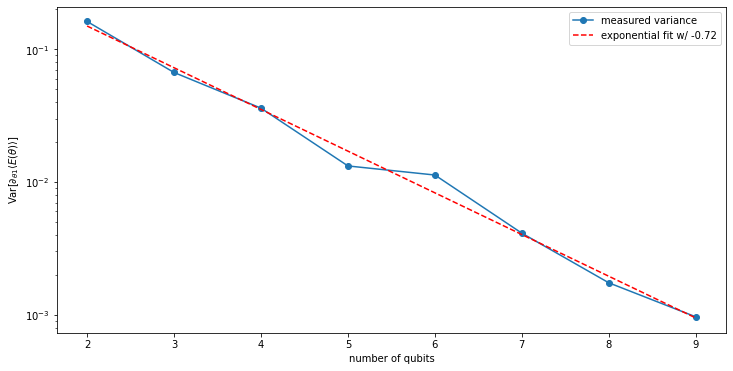
\includegraphics[width=\textwidth]{Artefact/Appendices/TwoLocalDefault.png}
    \centerline{b) TwoLocal Ansatz gradient variance values}
    \caption{
        The variances of gradient from differences ansatzes in the default configuration, the circuit is measured as a global cost function.
        For each iteration, we increase the qubit and repetition count by 1, starting from 2 to 9.
        The variances vanish exponentially to the number of qubits.
    }
    \label{Plot ansatzes variance default}
\end{figure}

In contrast, for the case of Local Cost Function and Shallow circuit, we observe that the variances of the ansatzes' gradient did not vanish when we attempt to increase the number of qubits.
This implies that the cost function landscape can sustain the slope.
Figure \ref{Plot ansatzes variance local cost} shows the result of the experiment for local cost function and shallow circuit.
We can see that the NLocal ansatz case produced a more steady graph compared to the TwoLocal ansatz, which mean the trainability of gradient-based optimization algorithms would be consistent.
For TwoLocal ansatz, we can see that the graph is more unstable, for example, the variance value for 7 qubits is higher compared to 4 or 9 qubits.

\begin{figure}
    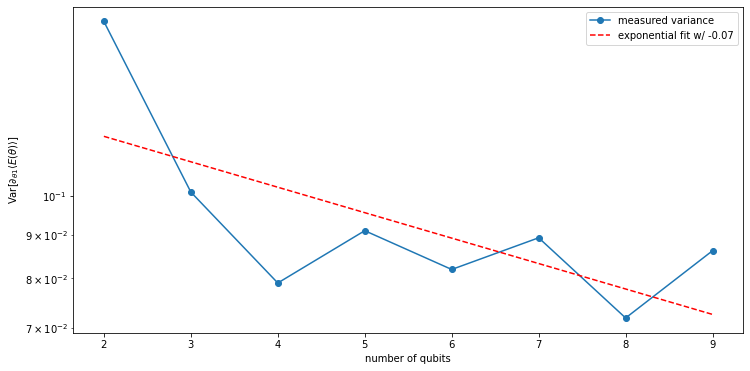
\includegraphics[width=\textwidth]{Artefact/Appendices/NLocalFixedLocal.png}
    \centerline{a) NLocal Ansatz gradient variance values}
    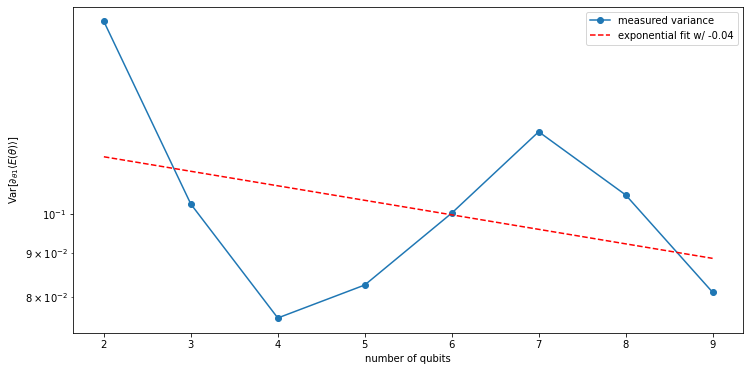
\includegraphics[width=\textwidth]{Artefact/Appendices/TwoLocalFixedLocal.png}
    \centerline{a) TwoLocal Ansatz gradient variance values}
    \caption{
        The variances of gradient from different ansatzes after applying a local cost function.
        We plot 2 to 9 qubits while keeping the repetition value fixed as 1. 
    }
    \label{Plot ansatzes variance local cost}
\end{figure}

\almarginpar{Very good presentation of results, however, perhaps individual descriptions could be close to the respective plots?}
To compare the effectiveness of the local cost function treatment, we plot the variance graph of above mention cases in figure \ref{Plot variance default and Local Cost}.
Overall, the ansatzes with the local cost function and restriction on circuit depth have their variance values remaining higher and being more consistent for higher qubit count, the ansatz with this treatment therefore would not possess a barren plateau.
On the other hand, the values for the default cases shrink exponentially and eventually, the near-zero gradient around the initial point will expand to a large plateau. 



\begin{figure}
    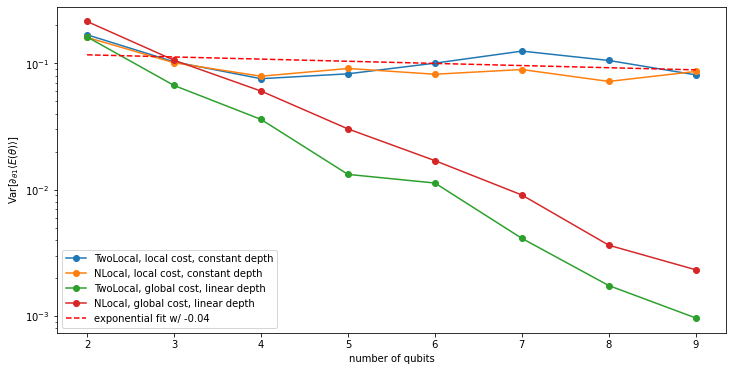
\includegraphics[width=\textwidth]{Artefact/Appendices/variancesLCF.png}
    \caption{
        Comparison of the variance values of the two ansatzes with and without Local Cost Function and constant depth.
        The ansatzes with Global Cost Function and increased depth have their gradient variances decay exponentially with the number of qubits. 
    }
    \label{Plot variance default and Local Cost}
\end{figure}

\almarginpar{We need some summary of the artefact section. What the minimum artefact shown? What aspects it did not address? What the full artefacts would still do?}
\almarginpar{Then we need the conclusion for the entire report. Has the research question been answered? If not what part was? Which objectives have been met? What work is still outstanding? Future work? Reflections?}
\almarginpar{Is 38 references sufficient for an hons thesis?}

*** Looks like we still need some more ***
